\chapter{Klasifikacijska točnost}
\label{ch:klasifikacijska-tocnost}

Sedaj ko vemo, kaj klasifikacijska drevesa so, se pojavi vprašanje, kakšna je točnost njihovih napovedi. Za začetek moramo definirati, kaj razumemo pod točnost. Najpreprostejša mera točnosti v klasifikaciji je klasifikacijska točnost, ki je izražena kot razmerje primerov, za katere je model pravilno napovedal razred. Poglejmo, če lahko ocenimo ali pa vsaj dobimo občutek za klasifikacijsko točnost z gradniki, ki jih že poznamo.

\begin{figure}[h]
    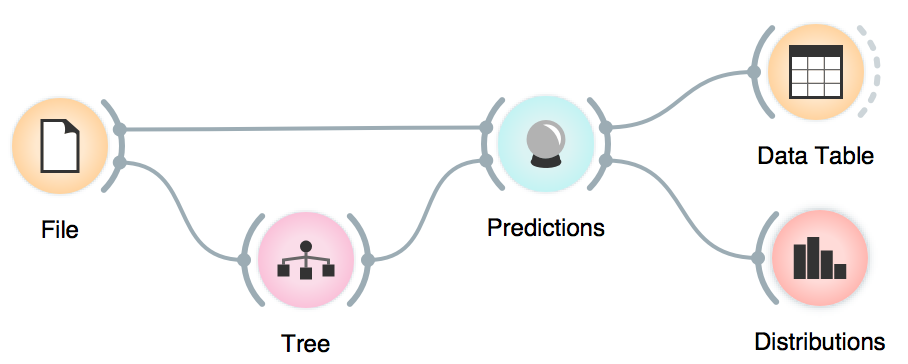
\includegraphics[width=0.9\linewidth]{workflow1.png}
    \caption{$\;$}
\end{figure}

\begin{wrapfigure}{o}{1.05\textwidth}
    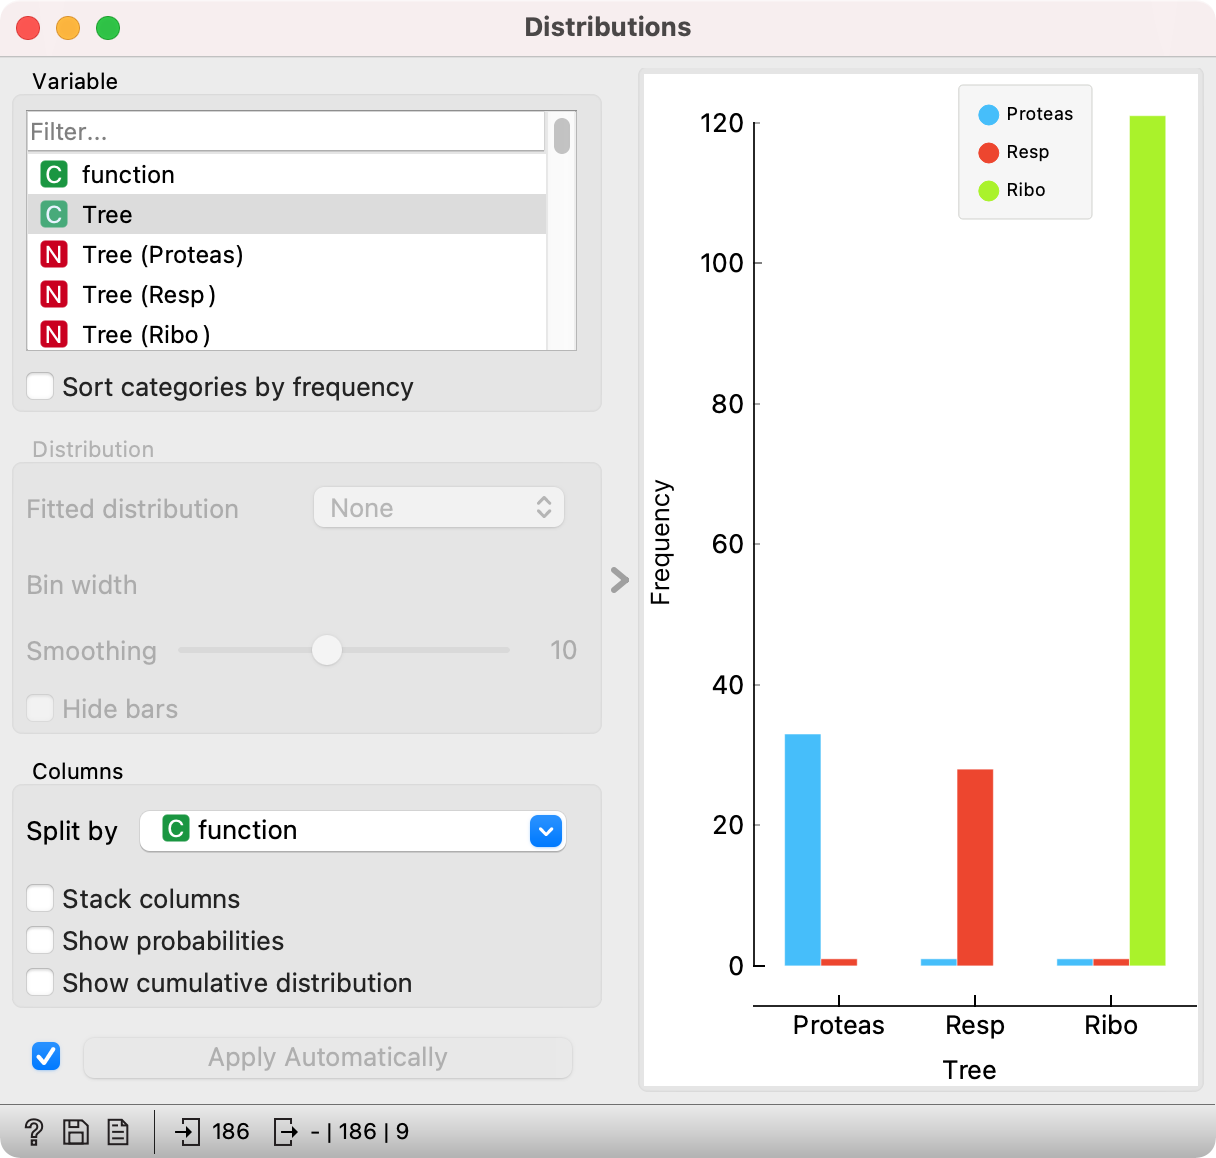
\includegraphics[scale=0.5]{distributions.png}
    \caption{$\;$}
\end{wrapfigure}

Predictions pošlje na izhod preglednico z dodanim stolpcem z napovedmi. V gradniku \widget{Data Table} lahko razvrstimo podatke po katerem koli od dveh stolpcev (Tree ali Function) in ročno izberemo primere, kjer sta vrednosti v stolpcih različni (kar bi bilo težavno na velikih podatkih). Če pravilno nastavimo spremenljivke, lahko v grobem ocenimo napovedno točnost kar v gradniku \widget{Distributions}.

\newpage
\clearpage

Včasih pa bi potrebovali kaj bolj natančnega kot zgolj grobo oceno iz Distributions gradnika. Statistiko pravilno in nepravilno klasificiranih primerov vidimo v matriki zmot (ang. \widget{Confusion Matrix}).

\begin{figure}[h]
    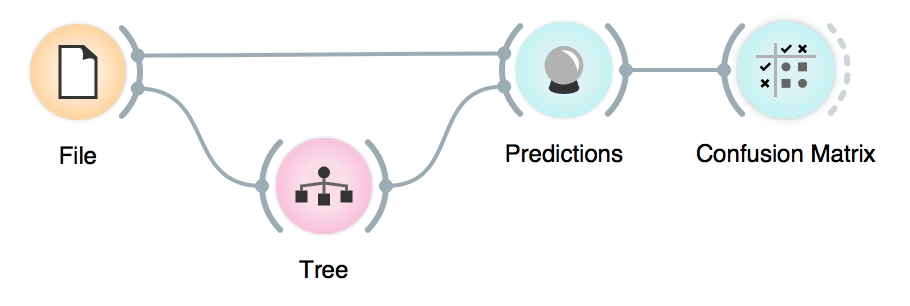
\includegraphics[width=0.9\linewidth]{workflow2.png}
    \caption{$\;$}
\end{figure}

\begin{figure*}[h]
    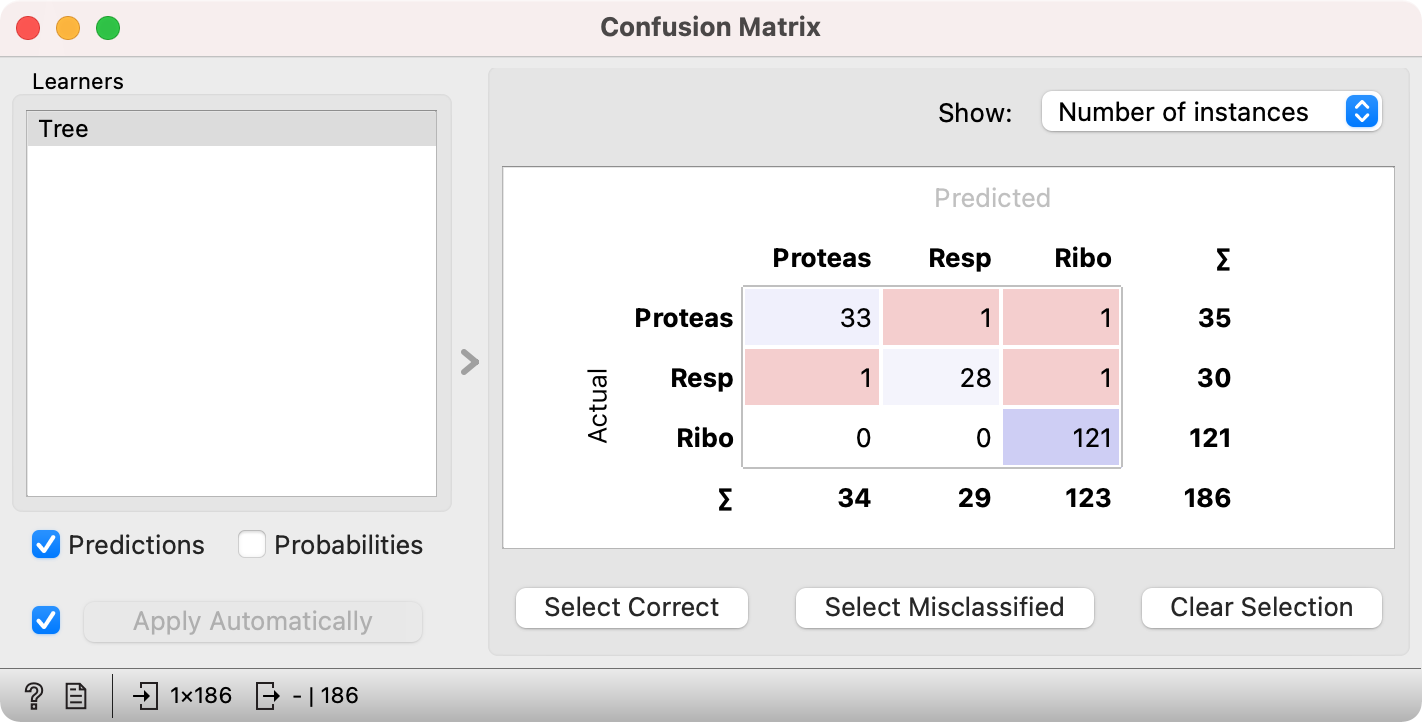
\includegraphics[width=0.7\linewidth]{confusion-matrix.png}
    \caption{$\;$}
\end{figure*}

Vidimo, da je drevo za 33 proteaz, 28 respiratornih genov in 121 ribosomov pravilno napovedalo rezultat. Vendar pa je napačno uvrstil 4 gene. Ker je klasifikacijska točnost razmerje pravilno napovedanih primerov, jo izračunamo kot število pravilnih napovedi (33 + 28 + 121 = 182) deljeno s številom vseh primerov (186). Klasifikacijska točnost je torej 182/186 =  97 \%. Sliši se dobro, pa je res?